\documentclass{article}
\usepackage[utf8]{inputenc}
\usepackage{emptypage}
\usepackage{pgfplots}
\usepackage{amssymb}
\usepackage{graphicx}
\usepackage{siunitx}
\usepackage{amsmath}
\usepackage{amsthm}
\usepackage[version=4]{mhchem}
\usepackage{hyperref}
\usepackage{array}
\usepackage{animate}
\usepackage{attachfile}
\usepackage{multirow}
\usepackage{breqn}
\usepackage{mathtools}
\usepackage{cancel}
\usepackage{fancyhdr}
\usepackage{afterpage}

\usepackage{listings}
\usepackage{color}

\definecolor{dkgreen}{rgb}{0,0.6,0}
\definecolor{gray}{rgb}{0.5,0.5,0.5}
\definecolor{mauve}{rgb}{0.58,0,0.82}

\lstset{frame=tb,
  language=MATLAB,
  aboveskip=3mm,
  belowskip=3mm,
  showstringspaces=false,
  columns=flexible,
  basicstyle={\small\ttfamily},
  numbers=none,
  numberstyle=\tiny\color{gray},
  keywordstyle=\color{blue},
  commentstyle=\color{dkgreen},
  stringstyle=\color{mauve},
  breaklines=true,
  breakatwhitespace=true,
  tabsize=3
}

\newcommand{\mysection}[2]{\setcounter{section}{#1}\addtocounter{section}{-1}\section{#2}}


\newcommand\blankpage{%
    \null
    \thispagestyle{empty}%
    \addtocounter{page}{-1}%
    \newpage}

% Clear off all default fancyhdr headers and footers
\fancyhf{}
% Put the page number at the right edge of odd pages, and left edge of even pages.
\fancyhead[RO,LE]{\thepage}
% Custom text at the left edge of odd pages, and right edge of odd pages.
\fancyhead[LO,RE]{\sffamily\itshape Flipped Classroom 1}
\pagestyle{fancy}

\usepackage{afterpage}

    
\begin{document}
 \pagenumbering{Roman}
\begin{titlepage}
	\clearpage\thispagestyle{empty}
	\center{
 
    }
	\vspace{2cm}

	
	\centering 
\includegraphics[scale=0.35]{Logo.png}
	
	
    	{\Huge Reliability Risk \& Safety Analysis \\ 
		\par}
		\vspace{1cm}

	{\Huge 
	\textbf{Flipped Classroom 1} \\
    }

	\vspace{1cm}
	{\Large
    	\textbf{Probability Exercises}\\
\vspace*{\fill}
}
	\vspace{1cm}
	{\Large \textbf{Group 7}}
 
Samuele Mezzaro\\ 
Simone Pagliuca\\
Cyrille de Lurion


\vspace*{\fill}

	
	\pagebreak

\end{titlepage}



\tableofcontents


\newpage
\pagenumbering{arabic}
\mysection{0}{States, Space of States and Events}
In an energy production plant there are 2 turbines: $T_a$ and $T_b$. \\
Each turbine can be in three different states:
\begin{itemize}
    \item 0: Operating
    \item 1: Degraded
    \item 2: Failed
\end{itemize}
Considering the following events:
\begin{itemize}
    \item A: $T_a$ has failed
    \item B: both turbines are degraded
    \item C: $T_b$ is not degraded
\end{itemize}
\subsection{Define the sample space $\Omega$ of the state of the turbines and represent it graphically}
\begin{figure}[h]
    \centering
    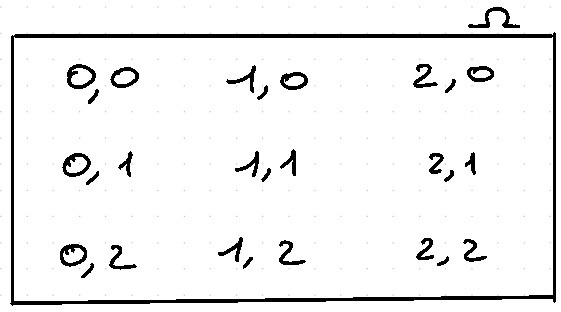
\includegraphics[width=0.5\linewidth]{image.png}

\end{figure}
\subsection{Represent events $A$, $B$ and $C$ in the sample space $\Omega$}
\begin{figure}[h]
    \centering
    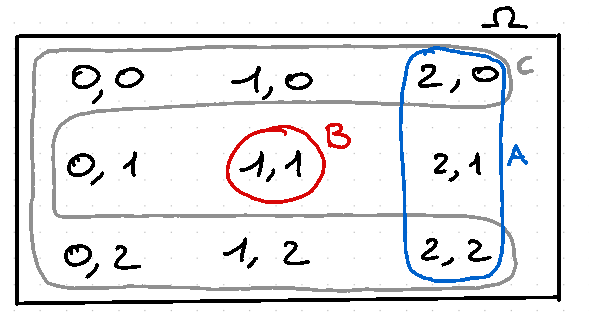
\includegraphics[width=0.5\linewidth]{image2.png}
    
    
\end{figure}

\newpage
\subsection{Find and represent $A \cap C$, $A \cup C$ and $(A \cap C)\cup B$}
\begin{figure}[h]
    \centering
    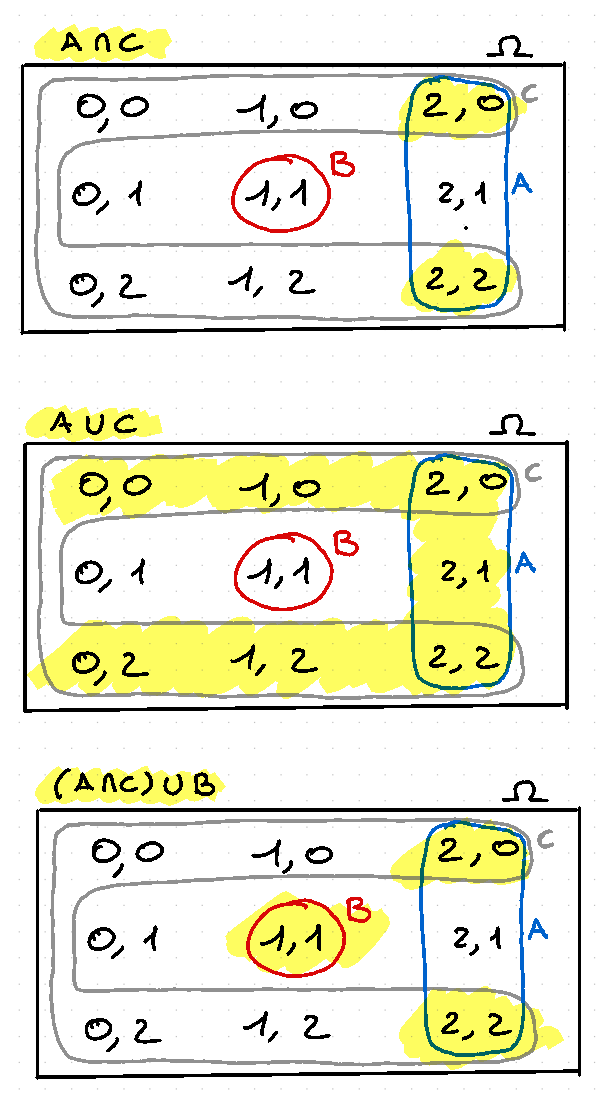
\includegraphics[width=0.5\linewidth]{image3.png}
    
    
\end{figure}



\newpage
\section{Combined Probability}
Consider a car headlight system composed of two taillights, $light_a$ and
$light_b$.
The probability that $light_b$ is failed is 0.045, the probability that $light_b$ is
failed is 0.055 and the probability that $light_a$ \textbf{OR} $light_b$ are failed is 0.070

$A$ = $ \text{ Event $light_a$ failed}$
$B$ = $\text{ Event $light_b$ failed}$

\subsection{What is the probability that both lights are failed?}
$P(A \cap B) = 0.045 +0.055-0.07 = 0.03 = 3\%$

\subsection{Are the two events statistically independent? If not, justify it from an engineering point of view.}
Given that the two lights are both wired to the same electric system of a car, we cannot expect an independent behaviour.

\subsection{Combined Probability $A|B$}
$P(A|B) = \frac{P(A \cap B)}{P(B)} = \frac{0.03}{0.055} = \frac{6}{11} = 54.54\%$

\subsection{Combined Probability $B|A$}
$P(A|B) = \frac{P(A \cap B)}{P(A)} = \frac{0.03}{0.045} = \frac{2}{3} = 66.67\%$

\subsection{Combined Probability $\bar A | \bar B$}
$P(\bar A| \bar B) = \frac{P(\bar A \cap \bar B)}{P(\bar B)} = \frac{1 - (0.055 + 0.045 - 0.03)}{1-0.055} = \frac{0.93}{0.945} = 98.41\%$

\newpage
\section{Two possible failure conditions}
A motor operated valve opens and closes intermittently on demand to control the
coolant level in an industrial process. An auxiliary battery pack is used to provide
power for approximately the $0.4\%$ of the time when there are plant power
outages. The demand failure probability of the valve is $4 \cdot 10^{-5}$ when operated
from the plant power and $8 \cdot 10^{-4}$ when operated from the battery pack.

\subsection{Find the demand failure probability?}
Assuming the number of demands is independent from the power source.\\
The probability of failure is $4 \cdot 10^{-5}$ for $99.6\%$ of the time, and $8 \cdot 10^{-4}$ for the remaining $0.4\%$
\begin{equation}
    P(fail) = \left( 1 - \frac{0.4}{100}\right) \cdot 4 \cdot 10^{-5} + \frac{0.4}{100}\cdot 8 \cdot 10^{-4}
\end{equation}
\begin{equation}
    P(fail) = 4.305 \cdot 10^{-5}
\end{equation}
\subsection{Is the increase due to the battery pack significant?.}
If the system is powered by the plant $100\%$ of the time, the failure probability is $4 \cdot 10^{-5}$, we can calculate the percentage difference:
\begin{equation}
    \Delta \% = \frac{4.305-4}{4} \cdot 100 = +7.6 \%
\end{equation}
Which might be a considerable increase.


\newpage
\section{Discrete probability distribution}
In an energy production plant, there are 5 pumps in parallel sharing a common
load. Let $X$ indicate the number of operating pumps. According to some
historical data, we assume that the following equation properly describes the
distribution of the number of working pumps:

\begin{figure}[h]
    \centering
    \centerline{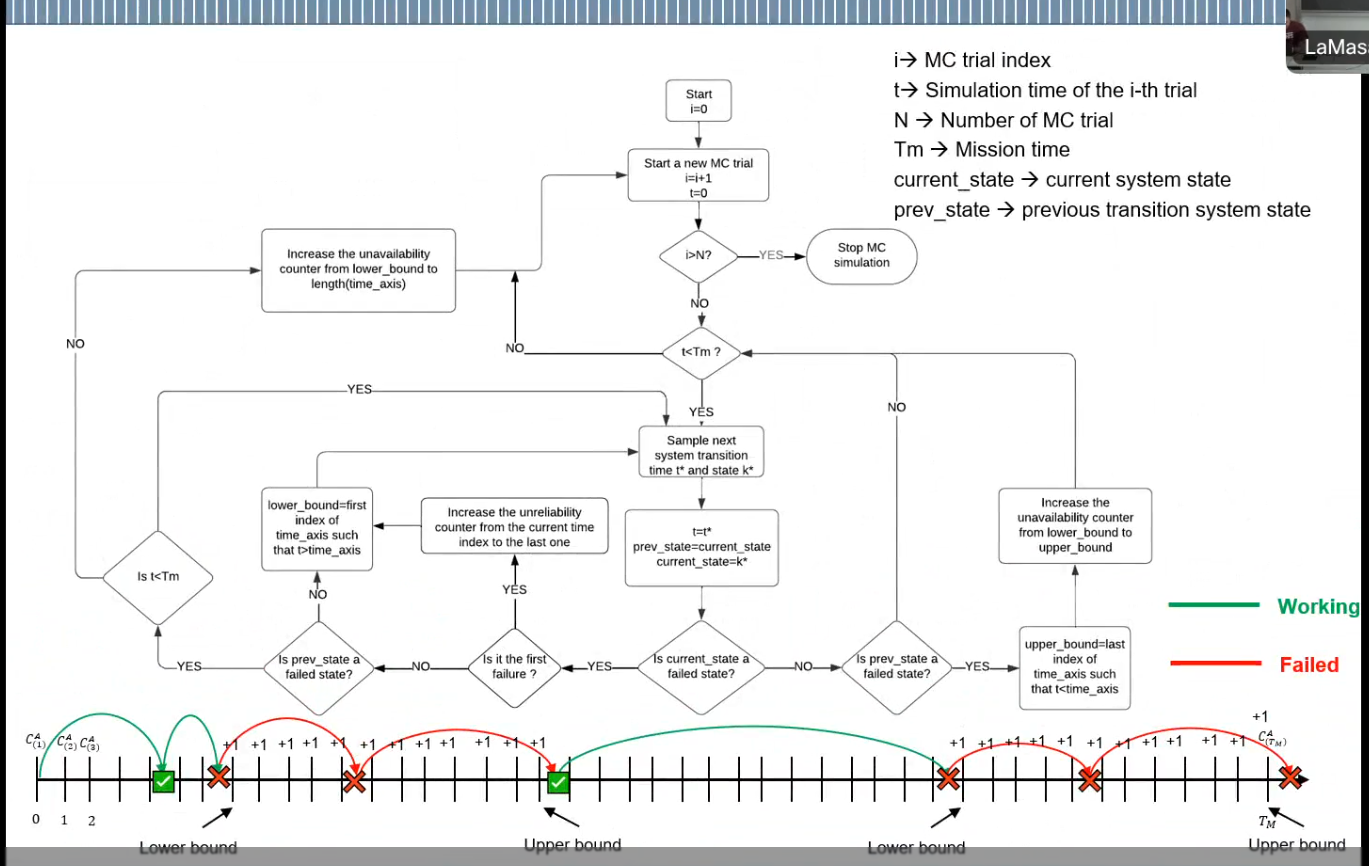
\includegraphics[scale=0.4]{Untitled.png}}
\end{figure}



\subsection{Compute A}
Given that the sum of the distribution shall equal 1, we can solve a simple equation to find the value of A: $\sum_{i=0}^{5} P(X=i) = A+A+A+3A+3A+3A = 1$, which gives $A = \frac{1}{12}$.

\begin{figure}[h]
    \centering
    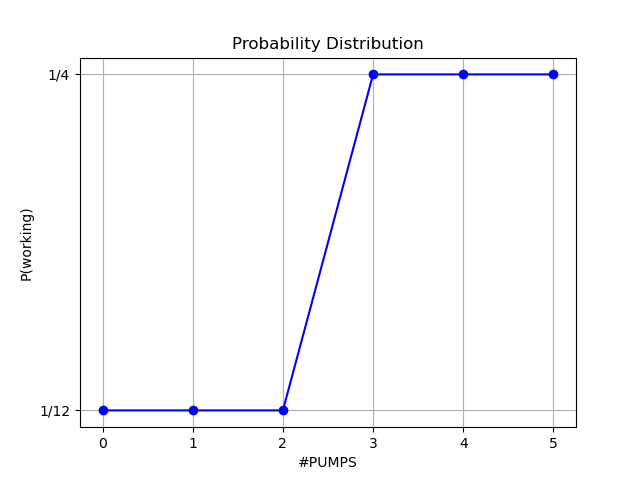
\includegraphics[width=0.5\linewidth]{Figure_3.png}
   
\end{figure}
\subsection{Probability that there are more then 2 operating pumps}
\begin{equation}
    P(>2) = 1 - P(2) - P(1) -P(0) = \frac{9}{12} = 0.75
\end{equation}


\subsection{Mean and Standard Deviation of X}
The mean number of working pumps is given by $\sum{P_i \cdot n_i}$, where $n$ refers to the number of working pumps. \\
The standard deviation is computed as $\sqrt{\sum{(n_i - mean)^2} \cdot P_i}$.
\begin{itemize}
    \item Mean = $3.25$
    \item $\sigma$ = $1.53$
\end{itemize}



\newpage
\section{Binomial Distribution}
In an electric system, there are 5 identical LED's operating independently.
The probability that an LED is operative after 1 year of operation is 70\%

\subsection{List possible combinations...}
\subsubsection{...of states with 0 LED's working after 1 year}
All of them are broken: $[0,0,0,0,0]$

\subsubsection{...of states with 1 LED's working after 1 year}
Just one is on (5 combinations): $[1,0,0,0,0]$, $[0,1,0,0,0]$, [...], $[0,0,0,0,1]$

\subsubsection{...of states with 3 LED's working after 1 year}
The number of possible combinations is given by the binomial factor $3 \choose 5 $ $= 10 $ possible combinations:

{\renewcommand{\arraystretch}{1.25}%
\setlength{\arrayrulewidth}{0.15mm}
    \begin{center}
    \begin{tabular}{|c|c|c|c|c|}
    \hline
         LED1&   LED2&LED3&LED4 &LED5\\
    \hline
        1&   1&1&0&0\\
    \hline
        0&   1&1&1&0\\
    \hline
         0&   0&1&1&1\\
    \hline
          1&   0&0&1&1\\
    \hline
          1&   1&0&0&1\\
    \hline
         1&   0&1&0&1\\
    \hline
 1& 1& 0& 1&0\\ \hline 
 0& 1& 1& 0&1\\ \hline 
 1& 0& 1& 1&0\\\hline
 0& 1& 0& 1&1\\\hline
    \end{tabular}
    \end{center}
}

\subsection{Probability only 3 LED's operating after 1 year}
Using binomial formula: ${n \choose k}p^k(1-p)^{(n-k)}$ with $n$ total number of LED's $n=5$, $k$ number of working LEDs $k=3$ and $p=0.7$ the probability of each LED's to be working after 1 year.
\begin{equation}
    P = {5 \choose 3 } \cdot 0.7 ^ 3 \cdot (1-0.7)^{(5-3)} = 30.87\%
\end{equation}

\subsection{Plot probability mass function (PMF) and cumulative distribution function (CDF)}
\begin{figure}[h]
    \centering
    \centerline{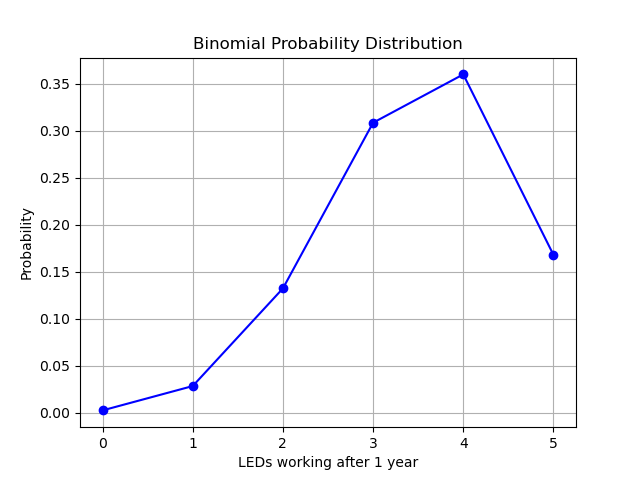
\includegraphics[scale=0.4]{4_a.png}}
\end{figure}
\begin{figure}[h]
    \centering
    \centerline{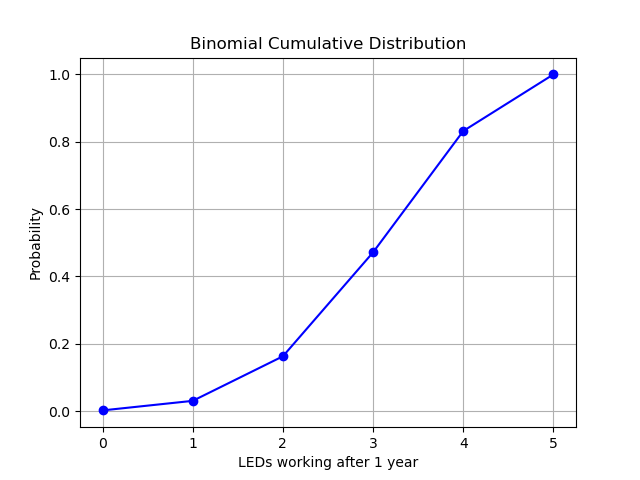
\includegraphics[scale=0.4]{4_b.png}}
\end{figure}


\subsection{Compute Mean, Var, $\sigma$}
The mean number of working LED's is given by $\sum{P_i \cdot n_i}$, where $n$ refers to the number of working LED's. \\
The variance is computed as $\sum{(n_i - mean)^2} \cdot P_i$, and the standard deviation is $\sigma = \sqrt{var}$.\\
\begin{itemize}
    \item Mean = $3.5$
    \item Var = $1.05$
    \item $\sigma$ = $1.0246$
\end{itemize}



\newpage
\section{Binomial Distribution 2}
There are 30,000 traffic lights in Chile. They are all based on the same
technology, and they have a single bulb. The probability that the bulb of a
traffic light fails during one month of service is $ p=0.003$.
At the beginning of March 2024, all traffic lights are properly working.
Also, the traffic department has in stock only 90 bulbs to replace failed
bulbs of traffic lights in all the country.

\subsection{Probability of more then 90 failures}
What is the probability that the
traffic department will not be able to replace a traffic light during the
period between the 1 st and 31 st of March? \\
We can compute the probability of having 90, or less failures over 30'000 traffic lights:
\begin{equation}
    P(fail \leq 90) = \sum_{k=0}^{90}{{k \choose 30000} \cdot (0.003)^k \cdot (1-0.003)^{30000-k}}
\end{equation}
And then the probability of shortage would be $P(fail>90) = 1 - P(fail \leq 90)$. \\
By using the following MATLAB code we can compute that $P(fail>90) = 47.20\%$


\subsection{How much stock to reduce the probability of not being able to replace}
How many traffic lights bulbs should the traffic department buy to
decrease the probability of having a shortage of traffic lights in the same
period of time to 0.001? \\
This can be solve by iteration over $k$ of the previous expression, while setting $P(fail) = 0.001$, with MATLAB we got $k=120$.
\begin{lstlisting}
p = 1 - sum(binopdf(0:90,30000,0.003));
k = 90; 
while p>0.001k = k+1;
p = 1 - binocdf(k,30000,0.003);
end
disp(k-1);
\end{lstlisting}

\newpage
\section{Rare, stochastic events}
The occurrences of earthquakes in region A may be modelled by a
Poisson process with constant rate of occurrence $\lambda$. Let $p(k; t, \lambda )$denote
the probability of $k$ earthquakes occurrences in $t$ years. \\
The mean occurrence rate of earthquakes in a certain region A is once
every 5 years. \\

For stochastic events that may occur in a continuous period of time the probability mass function is 
\begin{equation}
    p(k,t,\lambda)=\frac{(\lambda t)^k}{k!} e ^{-\lambda t}
\end{equation}

\subsection{Probability of no events in 10 years}
\begin{equation}
    p(0,10,\frac{1}{5}) = \cancelto{1}{(...)} e^{-\frac{1}{5}\cdot 10} = 0.1353 = 13.55\%
\end{equation}

\subsection{Probability of 1 event in 10 years}
\begin{equation}
    p(1,10,\frac{1}{5})= \frac{(\frac{1}{5} \cdot 10)^1}{1!}e^{-\frac{1}{5}\cdot 10}= 0.2707 = 27.07\%
\end{equation}

\subsection{Probability of more than 2 events in 10 years}
\begin{equation}
    p(>2,10,\frac{1}{5}) = 1 - p(2,10,\frac{1}{5}) - p(1,10,\frac{1}{5}) - p(0,10,\frac{1}{5}) 
\end{equation}
\begin{equation}
    p(>2,10,\frac{1}{5}) = 1 - \frac{(\frac{1}{5} \cdot 10)^2}{2!}e^{-\frac{1}{5}\cdot 10} - 0.2707 - 0.1353 = 0.3238 = 32.38 \%
\end{equation}

\newpage
\section{Rare, stochastic events 2}
The mean occurrence rate of extremely cold air events in a region is once
every 2 years. In case of extremely cold air events, the probability that the local power
supply system is seriously damaged is 0.03.

\subsection{Probability of no damage over 10-years period}
For stochastic events that may occur in a continuous period of time the probability mass function is 
\begin{equation}
    p(k,t,\lambda)=\frac{(\lambda t)^k}{k!} e ^{-\lambda t}
\end{equation}
In our case, no damage to the power grid $k=0$, over the span of 10 years $t=10$, and the probability of damage AND extreme cold air event, should be $\lambda = \frac{1}{2} \cdot 0.03 = 0.015$, therefore:
\begin{equation}
    p(0,10,0.015)=\frac{(0.015 \cdot 10)^0}{0!} e ^{-0.015 \cdot 10} = e ^{-0.015 \cdot 10} = 0.8607 = 86.07\%
\end{equation}

\subsection{Alternative method}
Let us denote :\\
C : random variable describing the number of times cold air arrives in 10 years in the region. C follows a Poisson law of parameter 5.\\
D : the event that the power system is severely damaged because of cold at the end of the 10 years period. The conditional probability of D occurring knowing that there was 1 wave of cold is 0.03 : $P(D|C=1)=0.03$.\\
X : the event that the power system is not seriously damaged because of cold at the end of the 10 years period.\\
\\
The events $P(C=i)$ for $i \in \mathbb{N}$ are a partition of the space into mutually exclusive and exhaustive events : $\sum_{i=0}^{+\infty} P(C=i) = 1$. So we can use the theorem of total probabilities to say that :
\begin{equation}
    P(X)=\sum_{i=0}^{+\infty} (1-P(D|C=i)) \times P(C=i)
\end{equation}
For a given event $C=i$, the power system can be damaged right away by the first cold wave with probability $0.03$, or by the second one if it was not damaged by the first one with probability $0.97 \times 0.03$, or by the third one if neither the first not the second waves damaged it with probability $0.97 \times 0.97 \times 0.03$... Since these events are mutually exclusive, the probability of their union is the some of the probabilities of the single events. In the end there is $P(D|C=i)=1-0.97^i$.
Eventually, the probability of X is:
\begin{equation}
    P(X)=\sum_{i=0}^{+\infty} 0.97^i \times \frac{5^i}{i!} e^{-5} = 86.07\%
\end{equation}

\end{document}
